% !TeX program = pdflatex

% Version modifiee : les parties 3, 5 et 6 sont integrees comme pages completes
% depuis le PDF exporte du PPT, afin de conserver au maximum le rendu original.
% Compilation : pdflatex main_modifie_embed.tex

\documentclass[aspectratio=169]{beamer}

\mode<presentation>
{
  \usetheme{default}
  \usecolortheme{default}
  \usefonttheme{default}
  \setbeamertemplate{navigation symbols}{}
  \setbeamertemplate{caption}[numbered]
  \setbeamertemplate{footline}{%
    \leavevmode%
    \hbox{%
      \begin{beamercolorbox}[wd=\paperwidth,ht=2.6ex,dp=1.2ex,rightskip=1.2em]{author in head/foot}%
        \hfill\usebeamerfont{author in head/foot}\insertframenumber
      \end{beamercolorbox}%
    }%
  }
}

\usepackage[french]{babel}
\usepackage[utf8]{inputenc}
\usepackage[T1]{fontenc}
\usepackage{lmodern}
\usepackage{amsmath}
\usepackage{amssymb}
\usepackage{graphicx}
\usepackage{booktabs}
\usepackage{ragged2e}
\usepackage{tikz}
\usepackage{pgfplots}
\usetikzlibrary{positioning,arrows.meta}
\pgfplotsset{compat=1.18}
\pgfplotsset{every axis/.append style={font=\scriptsize}}
\AtBeginEnvironment{frame}{\justifying}
\AtBeginEnvironment{block}{\justifying}
\AtBeginEnvironment{alertblock}{\justifying}
\AtBeginEnvironment{exampleblock}{\justifying}
\addtobeamertemplate{itemize/enumerate body begin}{\justifying}{}
\addtobeamertemplate{itemize/enumerate subbody begin}{\justifying}{}
\addtobeamertemplate{itemize/enumerate subsubbody begin}{\justifying}{}

\newcommand{\PPTFullSlide}[1]{%
  {%
    \setbeamertemplate{background}{%
      \includegraphics[page=#1,width=\paperwidth,height=\paperheight]{slides/rapport_sections_3_5_6_presentation.pdf}%
    }%
    \begin{frame}[plain]
      \begin{tikzpicture}[remember picture,overlay]
        \node[
          anchor=south east,
          xshift=-0.18cm,
          yshift=0.18cm,
          rounded corners=2pt,
          fill=white,
          fill opacity=0.85,
          text opacity=1,
          inner xsep=4pt,
          inner ysep=2pt,
          font=\scriptsize
        ] at (current page.south east) {\insertframenumber};
      \end{tikzpicture}
    \end{frame}%
  }%
}

\title[Rapport S2]{MLP pour MNIST et moteur de différentiation automatique\\Extensions S2 : GEMM, CNN, Tiny-ImageNet et MPI}
\author[Jianye Shi et al.]{Jianye Shi \and Hao Qian \and Xiang Bian \and Abdennour Boulmis}
\institute[UVSQ]{Master CHPS -- UVSQ\\Encadrement : Aurélien Delval}
\date{6 mai 2026}

\begin{document}

\begin{frame}
  \titlepage
\end{frame}

\section{Introduction}

\begin{frame}{1. Introduction}
\small
\begin{itemize}
  \item Point de départ : un prototype MNIST avec un MLP, de l'autodiff en mode reverse et une boucle d'entraînement.
  \item Objectif du semestre : élargir ce prototype vers un système expérimental plus complet.
  \item Trois directions :
  \begin{itemize}
    \item GEMM et convolution pour le calcul bas niveau ;
    \item modèles et données plus exigeants, avec CNN (puis ResNet) et Tiny-ImageNet ;
    \item entraînement distribué avec MPI, puis chemin inspiré d'IST-DP.
  \end{itemize}
\end{itemize}

\begin{alertblock}{Idée centrale}
Le même runtime d'entraînement doit rester réutilisable quand on change à la fois d'opérateurs, de modèles, de données et de mode d'exécution.
\end{alertblock}

\end{frame}
\section{Optimisation GEMM}

\begin{frame}{2. GEMM : méthodologie et environnement}
\scriptsize
\begin{columns}[T,totalwidth=\textwidth]
\column{0.52\textwidth}
\begin{block}{Pourquoi commencer par GEMM ?}
\begin{itemize}
  \item GEMM est l'opérateur central des couches fully connected.
  \item Le chemin convolutif \texttt{im2col + GEMM} dépend aussi directement de sa performance.
\end{itemize}
\end{block}

\begin{block}{Implémentations comparées}
\begin{itemize}
  \item \texttt{blas}, \texttt{omp}, \texttt{omp\_blocked}, \texttt{omp\_blocked\_packb}, \texttt{omp\_blocked\_packab}, \texttt{omp\_gotoblas\_avx2}, \texttt{omp\_gotoblas\_avx512}
  \item Les workloads viennent de formes réelles du projet : couches MLP et CNN, pas uniquement des matrices synthétiques.
\end{itemize}
\end{block}

\column{0.44\textwidth}
\begin{block}{Protocole / environnement}
\begin{itemize}
  \item Plateforme contrôlée : Ryzen 9 8940HX, fréquence fixée, OpenBLAS + OpenMP
  \item Comparaisons limitées à 1--8 threads physiques, avec \texttt{OMP\_PROC\_BIND=true} et \texttt{OMP\_PLACES=cores}
  \item Restriction expérimentale à 8 CPU physiques via \texttt{taskset -c 0-7}
  \item 5 warm-up, puis 2000 fois répétées avec médiane du temps
  \item SMT désactivé : sur GEMM, les threads logiques se partagent les mêmes unités d'exécution, avec peu de gain et plus d'interférences.
\end{itemize}
\end{block}

\end{columns}
\end{frame}
\begin{frame}{2. GEMM : définitions des implémentations}
\scriptsize
\begin{columns}[T,totalwidth=\textwidth]
\column{0.62\textwidth}
\begin{itemize}
  \item \texttt{blas} : appel à OpenBLAS, utilisé comme référence externe.
  \item \texttt{omp} : version OpenMP de base, sans blocking structuré ni packing.
  \item \texttt{omp\_blocked} : ajout d'un blocking cache pour améliorer la réutilisation des sous-blocs (\texttt{BlockSize}=64).
  \item \texttt{omp\_blocked\_packb} : blocking + packing du panneau \(B\) seulement (\texttt{BlockSize}=48).
  \item \texttt{omp\_blocked\_packab} : blocking + packing explicite des panneaux de \(A\) et \(B\) (\texttt{PackM}=32, \texttt{PackN}=128, \texttt{PackK}=16).
  \item \texttt{omp\_gotoblas\_avx2} : organisation de type GotoBLAS avec micro-kernel AVX2 en \texttt{float32} (\texttt{\_mm256\_loadu\_ps}, broadcast, FMA).
  \item \texttt{omp\_gotoblas\_avx512} : même principe général, avec micro-kernel AVX-512 (par défaut \texttt{avx512\_8x32}), unroll \(\times 4\) de la boucle \(K\) (directive compilateur, pas déroulage manuel complet) et prefetch explicite des données packées.
\end{itemize}

\column{0.35\textwidth}
\centering
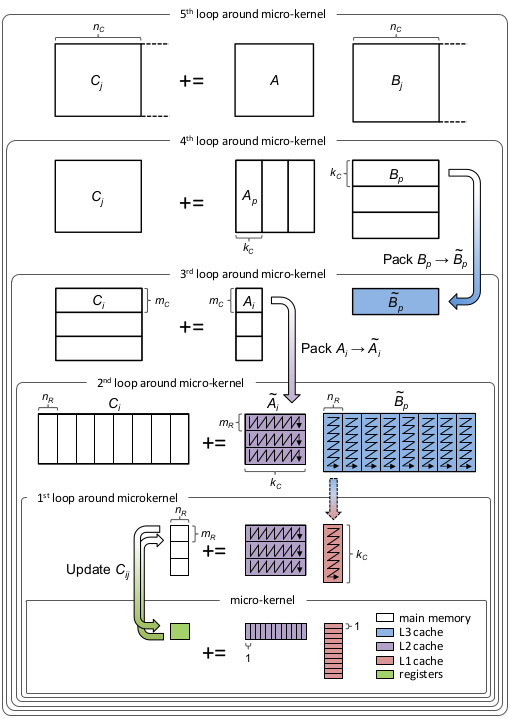
\includegraphics[width=\textwidth,height=0.90\textheight,keepaspectratio]{Images/blis_design.png}
\end{columns}
\end{frame}

\begin{frame}{2. GEMM : organisation GotoBLAS}
\scriptsize
\begin{columns}[T,totalwidth=\textwidth]
\column{0.50\textwidth}
\vspace{0.3cm}
\begin{itemize}
  \item Schéma conceptuel : $C_r$ dans les registres ; $A_r/B_r$ au plus près du micro-kernel ; $A_c$ plutôt orienté cache privé, $B_c$ plutôt orienté cache partagé.
  \item Le packing régularise les accès. Cette lecture guide les paramètres, sans supposer une résidence stricte et permanente de chaque bloc dans un niveau de cache donné.
  \item Configuration fixe retenue : \texttt{avx2\_8x8}, $K_c=384$, \texttt{kCacheBlockM}$=8$ (soit $M_c$ effectif $=64$), $N_c=448$. Le détail du réglage figure en annexe.
\end{itemize}
\centering

\column{0.47\textwidth}
\centering

\includegraphics[width=\textwidth,height=0.90\textheight,keepaspectratio]{Images/DataMovement.png}
\end{columns}
\end{frame}

\begin{frame}{2. GEMM : résultats de montée en charge (256x256)}
\scriptsize
\begin{columns}[T,totalwidth=\textwidth]
\column{0.62\textwidth}
\centering
\includegraphics[width=\textwidth,height=0.70\textheight,keepaspectratio]{Images/scaling_plot_256_only.png}

\column{0.35\textwidth}
\begin{itemize}
  \item Ici on fixe une seule taille synthétique, \(256 \times 256\), et on compare les temps de 1 à 8 threads.
  \item Le blocking et le packing améliorent déjà nettement la base \texttt{omp}.
  \item Les chemins \texttt{omp\_gotoblas\_avx2} et la variante AVX-512 descendent plus vite avec le nombre de threads.
  \item À 8 threads sur ce cas, OpenBLAS reste le plus rapide, mais l'écart avec les variantes GotoBLAS devient beaucoup plus faible.
\end{itemize}
\end{columns}
\end{frame}

\section{Loss et optimisateurs}

% Partie 3 remplacee par les 2 pages originales du PPT.
\PPTFullSlide{1}
\PPTFullSlide{2}

\section{Convolution}

\begin{frame}{4. Opérateur de convolution : pipeline}
\scriptsize
\begin{columns}[T,totalwidth=\textwidth]
\column{0.46\textwidth}
\centering
\begin{tikzpicture}[
  box/.style={draw, rounded corners=2pt, align=center, minimum width=2.3cm, minimum height=0.9cm, fill=gray!8},
  arr/.style={-{Latex[length=2mm]}, line width=0.8pt}
]
\node[box] (in) {Entrée\\$(N,C,H,W)$};
\node[box, below=0.45cm of in] (im2col) {\texttt{im2col}};
\node[box, below=0.45cm of im2col] (gemm) {GEMM};
\node[box, below=0.45cm of gemm] (out) {Sortie / gradients};
\draw[arr] (in) -- (im2col);
\draw[arr] (im2col) -- node[right, font=\scriptsize] {$X_{col}$} (gemm);
\draw[arr] (gemm) -- node[right, font=\scriptsize] {$Y=W_{col}X_{col}$} (out);
\end{tikzpicture}

\column{0.5\textwidth}
\begin{itemize}
  \item Le backend convolutif implémente la chaîne \texttt{im2col $\rightarrow$ GEMM $\rightarrow$ reshape}.
  \item Cette factorisation permet de réutiliser un noyau GEMM déjà optimisé.
  \item En rétropropagation, \texttt{col2im} reconstruit le gradient par rapport à l'entrée.
  \item Le coût d'exécution ne se limite pas à GEMM :
  \begin{itemize}
    \item transformations de données
    \item mouvements mémoire
  \end{itemize}
\end{itemize}

\end{columns}
\end{frame}

\begin{frame}{4. Opérateur de convolution : optimisations}
\scriptsize
\begin{itemize}
  \item \textbf{Parallélisation}
  \begin{itemize}
    \item Découpage par sorties indépendantes
    \item Réduction des conflits d'écriture et du coût de synchronisation
  \end{itemize}
  \item \textbf{Accès mémoire}
  \begin{itemize}
    \item Réorganisation des boucles \texttt{im2col}/\texttt{col2im}
    \item Accès plus continus, meilleure localité cache, latence plus stable
  \end{itemize}
  \item \textbf{Buffers temporaires}
  \begin{itemize}
    \item Réutilisation des buffers intermédiaires
    \item Diminution des allocations/libérations répétées
  \end{itemize}
  \item \textbf{Observation expérimentale}
  \begin{itemize}
    \item Gains plus marqués pour des charges moyennes à élevées
    \item Gains limités pour de petites charges (coût fixe du parallélisme)
  \end{itemize}
\end{itemize}
\end{frame}

\section{Architecture CNN}

% Partie 5 remplacee par les 4 pages originales du PPT.
\PPTFullSlide{3}
\PPTFullSlide{4}
\PPTFullSlide{5}
\PPTFullSlide{6}

\section{Optuna}

% Partie 6 remplacee par la page originale du PPT.
\PPTFullSlide{7}

\section{Tiny-ImageNet}

\begin{frame}{7. Tiny-ImageNet : montée en complexité}
\small
\begin{columns}[T,totalwidth=\textwidth]
\column{0.46\textwidth}
\centering
\begin{tikzpicture}[
  box/.style={draw, rounded corners=2pt, align=center, minimum width=2.4cm, minimum height=0.9cm, fill=gray!8},
  arr/.style={-{Latex[length=2mm]}, line width=0.8pt}
]
\node[box] (disk) {JPEG sur disque};
\node[box, below=0.45cm of disk] (batchsource) {\texttt{BatchSource}};
\node[box, below=0.45cm of batchsource] (loader) {Chargement / décodage\\par batch};
\node[box, below=0.45cm of loader] (train) {CNN / ResNet};
\draw[arr] (disk) -- (batchsource);
\draw[arr] (batchsource) -- (loader);
\draw[arr] (loader) -- (train);
\end{tikzpicture}

\column{0.5\textwidth}
\begin{itemize}
  \item Tiny-ImageNet: 200 classes, images RGB $64\times64$ (3 canaux).
  \item Entraînement: $\sim$100\,000 images (environ 500 / classe).
  \item Validation: 10\,000 images (50 / classe).
  \item Par rapport à MNIST: plus de classes, données couleur, variabilité visuelle plus forte.
  \item Objectif de cette étape: valider le passage à l'échelle du pipeline C++.
\end{itemize}
\end{columns}
\end{frame}

\begin{frame}{7. Tiny-ImageNet : résultat d'ingénierie}
\scriptsize
\begin{columns}[T,totalwidth=\textwidth]
\column{0.62\textwidth}
\centering
\begin{tikzpicture}
\begin{axis}[
  width=\textwidth,
  height=0.50\textheight,
  xmin=1, xmax=40,
  ymin=0, ymax=50,
  xlabel={Epoch},
  ylabel={Précision (\%)},
  xtick={1,5,10,20,30,40},
  ymajorgrids=true,
  grid style={gray!20},
  legend style={draw=none, fill=none, font=\scriptsize, at={(0.02,0.98)}, anchor=north west}
]
\addplot[color=teal!70!black, line width=1.1pt, mark=*, mark size=2pt] coordinates {
  (1,0.87) (5,7.69) (10,16.56) (20,30.96) (30,41.50) (40,47.33)
};
\addlegendentry{Train}
\addplot[color=red!75!black, line width=1.1pt, mark=triangle*, mark size=2.4pt] coordinates {
  (1,1.54) (5,8.46) (10,11.56) (20,9.49) (30,7.77) (40,7.24)
};
\addlegendentry{Validation}
\end{axis}
\end{tikzpicture}

\column{0.35\textwidth}
\begin{itemize}
  \item Le pipeline Tiny-ImageNet est opérationnel dans le framework.
  \item La boucle d'entraînement reste la même (chargement, labels, optimisation).
  \item Les résultats actuels montrent un écart train/validation marqué.
  \item Le point principal ici est la faisabilité système, pas l'accuracy finale.
\end{itemize}

\medskip
\textbf{Lecture.} L'étape valide l'intégration Tiny-ImageNet; l'amélioration de la précision et du coût d'entraînement relève de la phase suivante (architecture, régularisation, tuning).
\end{columns}
\end{frame}

\section{Entraînement distribué}

\begin{frame}{8. Entraînement distribué : organisation}
\scriptsize
\centering
\begin{tikzpicture}[
  box/.style={draw, rounded corners=2pt, align=center, minimum height=1.1cm, fill=gray!8},
  arr/.style={-{Latex[length=2mm]}, line width=0.8pt}
]
\node[box, minimum width=2.8cm] (r0) {Rank $r$\\forward + backward local};
\node[box, right=0.55cm of r0, minimum width=2.8cm] (sync) {Synchronisation\\des gradients};
\node[box, right=0.55cm of sync, minimum width=2.8cm] (step) {Mise à jour\\des paramètres};
\draw[arr] (r0) -- (sync);
\draw[arr] (sync) -- (step);

\node[box, below=1.0cm of r0, minimum width=2.65cm] (p1) {paramètre\\par paramètre\\{\tiny 1 AllReduce / paramètre}};
\node[box, right=0.35cm of p1, minimum width=2.55cm] (p2) {bucketed\\{\tiny regrouper plusieurs gradients}};
\node[box, right=0.35cm of p2, minimum width=2.55cm] (p3) {overlap\\{\tiny communiquer pendant le backward}};
\node[box, right=0.35cm of p3, minimum width=2.7cm] (p4) {compression\\{\tiny compresser avant AllReduce}};
\draw[arr] (p1) -- (p2);
\draw[arr] (p2) -- (p3);
\draw[arr] (p3) -- (p4);
\end{tikzpicture}

\vspace{0.15cm}
\begin{itemize}
  \item Le schéma mathématique ne change pas : on reste en data parallel synchrone,
  \[
  g_{\text{global}}=\frac{1}{B_{\text{global}}}\sum_r g_r
  \]
  \item \texttt{bucketed} réduit le nombre d'appels collectifs ; \texttt{overlap} cherche à masquer \texttt{sync\_wait} ; \texttt{compression} vise à réduire le payload.
\end{itemize}
\end{frame}


\begin{frame}{8. Entraînement distribué : résultats}
\small
\centering
\includegraphics[width=0.68\textwidth]{Images/mpi_scaling_fixed_global_batch.png}

\vspace{0.05cm}
\tiny
\textit{Strong scaling : \texttt{global\_batch=128} fixé, \texttt{local\_batch=128/np}, seed=42.}\\
Speedup : $1.00\times \to 1.82\times \to 3.90\times$

\vspace{0.15cm}
\begin{itemize}
  \item \textbf{Strong scaling} (\texttt{global\_batch=128} fixé) : même nombre de steps ($\approx$469) pour tout \texttt{np} ; speedup $3.90\times$ à \texttt{np=4} — quasi-idéal car MPI en mémoire partagée (machine unique), pas sur réseau.
\end{itemize}

\end{frame}

\section{IST}

\begin{frame}{9. IST : motivation et principe}
\scriptsize
\begin{columns}[T,totalwidth=\textwidth]
\column{0.50\textwidth}
\begin{block}{Point de départ}
\begin{itemize}
  \item Ce n'est pas l'IST complet de l'article.
  \item En data parallel classique : synchronisation à chaque step.
  \item Quand le nombre de workers augmente, cette synchronisation devient coûteuse.
\end{itemize}
\end{block}

\begin{alertblock}{Idée}
Synchroniser moins souvent, sans changer toute la boucle d'entraînement.
\end{alertblock}

\column{0.46\textwidth}
\centering
\begin{tikzpicture}[
  box/.style={draw, rounded corners=2pt, align=center, minimum width=2.45cm, minimum height=0.62cm, fill=gray!8},
  arr/.style={-{Latex[length=2mm]}, line width=0.7pt}
]
\node[box] (copy) {Copie complète\\du modèle};
\node[box, below=0.35cm of copy] (fb) {Forward / backward\\inchangés};
\node[box, below=0.35cm of fb] (mask) {Mask par rank};
\node[box, below=0.35cm of mask] (local) {Updates locaux\\pendant $K$ steps};
\node[box, below=0.35cm of local] (sync) {Fusion\\\texttt{MPI\_Allreduce}};
\draw[arr] (copy) -- (fb);
\draw[arr] (fb) -- (mask);
\draw[arr] (mask) -- (local);
\draw[arr] (local) -- (sync);
\end{tikzpicture}

\vspace{0.15cm}
\textbf{Deux notions à retenir}
\begin{itemize}
  \item \textbf{Mask} : paramètres modifiables par un rank.
  \item \textbf{$K$} : nombre de steps locaux avant synchronisation.
\end{itemize}
\end{columns}
\end{frame}

\begin{frame}{9. IST : fenêtre locale et validation}
\scriptsize
\begin{columns}[T,totalwidth=\textwidth]
\column{0.53\textwidth}
\begin{block}{Pendant la fenêtre locale}
\begin{itemize}
  \item chaque rank ne met à jour que sa partie des paramètres
  \item si $K$ augmente : moins de synchronisations
  \item risque : modèles locaux trop différents si la fenêtre est trop longue
  \item fin de fenêtre : fusion des changements via \texttt{MPI\_Allreduce}
\end{itemize}
\end{block}

\begin{alertblock}{Limite à rappeler}
\begin{itemize}
  \item communication encore dense
  \item gain surtout lié à la baisse de fréquence de synchronisation
\end{itemize}
\end{alertblock}

\column{0.43\textwidth}
\begin{block}{Expériences}
\begin{itemize}
  \item tests sur le cluster \texttt{zen.univ-lille.fr}
  \item plusieurs ranks MPI
  \item objectif : vérifier le fonctionnement distribué réel
  \item ablation sur $K$ : meilleur compromis observé avec $K=4$
\end{itemize}
\end{block}

\medskip
\centering
\begin{tabular}{lcc}
\toprule
Mode & Acc. val. & Temps \\
\midrule
dense & 3.51\% & 243 s \\
IST $K=1$ & 3.51\% & 243 s \\
IST $K=4$ & 4.33\% & 244 s \\
\bottomrule
\end{tabular}

\vspace{0.15cm}
\textit{Tiny-ImageNet, seed=42, 1 epoch, world\_size=2.}
\end{columns}
\end{frame}

\begin{frame}{9. Chemin inspiré d'IST : strong scaling}
\scriptsize
\begin{columns}[T,totalwidth=\textwidth]
\column{0.62\textwidth}
\centering
\begin{tikzpicture}
\begin{axis}[
  width=\textwidth,
  height=0.58\textheight,
  xmin=1, xmax=8,
  ymin=0, ymax=370,
  xlabel={World size},
  ylabel={Temps par epoch (s)},
  xtick={1,2,4,8},
  ymajorgrids=true,
  grid style={gray!20},
  legend style={draw=none, fill=none, font=\scriptsize, at={(0.98,0.98)}, anchor=north east}
]
\addplot[color=blue!65, line width=1.1pt, mark=*, mark size=2.2pt] coordinates {
  (1,343.287) (2,179.300) (4,89.970) (8,58.425)
};
\addlegendentry{Mesuré}
\addplot[color=gray!75, line width=1.0pt, dashed, mark=square*, mark size=2pt] coordinates {
  (1,343.287) (2,171.643) (4,85.822) (8,42.911)
};
\addlegendentry{Idéal}
\end{axis}
\end{tikzpicture}

\vspace{0.05cm}
\textit{Speedup : $1.00\times \rightarrow 1.91\times \rightarrow 3.82\times \rightarrow 5.88\times$}

\column{0.35\textwidth}
\begin{block}{Protocole}
\begin{itemize}
  \item Tiny-ImageNet, CNN
  \item IST avec $K=4$
  \item \texttt{global\_batch}=256 fixé
  \item \texttt{local\_batch}=256/\texttt{world\_size}
\end{itemize}
\end{block}

\begin{block}{Lecture}
\begin{itemize}
  \item temps : 343 s $\rightarrow$ 58 s
  \item scaling proche de l'idéal jusqu'à 4 workers
  \item à 8 workers, le temps baisse encore mais l'efficacité diminue
\end{itemize}
\end{block}

\medskip
\textbf{Conclusion.} Le chemin IST fonctionne avec MPI sur cluster et montre un potentiel de passage à l'échelle.
\end{columns}
\end{frame}

\section{Conclusion}

\begin{frame}{Bilan}
\small
\begin{itemize}
  \item Le backend GEMM a été clarifié, comparé et stabilisé pour servir de base aux expériences suivantes.
  \item Le projet dépasse désormais le seul cas MLP/MNIST : CNN, ResNet, Tiny-ImageNet et MPI sont intégrés dans un même runtime.
  \item Les chemins distribués couvrent déjà bucketed, un overlap\_bucketed correctness-only, la compression côté runtime et une variante inspirée d'IST encore expérimentale.
  \item Les prochaines priorités sont claires : convolution plus efficace, pipeline d'entrée plus riche, meilleure généralisation sur Tiny-ImageNet et communication plus creuse côté IST.
\end{itemize}

\vfill
\centering
\Large Questions
\end{frame}

\appendix
\section{Annexe Cluster}

\begin{frame}{Annexe : configuration cluster}
\footnotesize
\begin{columns}[T,onlytextwidth]
\column{0.49\textwidth}
\begin{block}{Nœud et pile}
\begin{itemize}
  \item \texttt{zen.univ-lille.fr}, exécution Slurm via \texttt{sbatch}
  \item 2 \(\times\) \texttt{AMD EPYC 9354} : 64 cœurs physiques, 128 CPU logiques
  \item 2 domaines NUMA ; SIMD : FMA, AVX2, AVX-512
  \item caches (\texttt{lscpu}) : L1d/L1i 32 KB, L2 1 MB, L3 32 MB
  \item modules : \texttt{gcc/13.2.0}, \texttt{openblas/0.3.24}, \texttt{openmpi/4.1.6}
\end{itemize}
\end{block}

\column{0.49\textwidth}
\begin{block}{Ressources et protocole}
\begin{itemize}
  \item validation IST : 1 nœud, 2 ranks MPI, 1 CPU par rank
  \item sweep scaling : 1 nœud, jusqu'à 8 ranks MPI, 1 CPU par rank
  \item runs intra-nœud uniquement : pas de coût réseau inter-nœuds
  \item Tiny-ImageNet, batch 64, learning rate 0.01
  \item IST : \(K \in \{1,4\}\), seeds \(42/43/44\), runs de 1 à 2 epochs
\end{itemize}
\end{block}
\end{columns}
\end{frame}

\begin{frame}{Annexe : dense vs IST \(K=4\)}
\footnotesize
\textbf{\large Synthèse multi-seed}

\vspace{0.10cm}
\begin{columns}[T,onlytextwidth]
\column{0.49\textwidth}
\centering
\textbf{Gain précision vs dense (pp)}

\begin{tikzpicture}
\begin{axis}[
  width=\linewidth,
  height=0.62\textheight,
  ybar,
  bar width=9pt,
  ymin=-1.0, ymax=1.05,
  ylabel={$\Delta$ acc.},
  symbolic x coords={1/42,1/43,1/44,2/42,2/43,2/44},
  xtick=data,
  enlarge x limits=0.10,
  ymajorgrids=true,
  grid style={gray!20},
  axis x line*=bottom,
  axis y line*=left,
  xticklabel style={rotate=45, anchor=east, font=\scriptsize},
  tick label style={font=\scriptsize},
  nodes near coords,
  every node near coord/.append style={font=\tiny, anchor=south}
]
\addplot[draw=teal!80!black, fill=teal!55] coordinates {
  (1/42,0.82) (1/43,0.16) (1/44,0.25)
  (2/42,0.23) (2/43,0.61) (2/44,-0.70)
};
\end{axis}
\end{tikzpicture}

\column{0.49\textwidth}
\centering
\textbf{Gain temps vs dense (\%)}

\begin{tikzpicture}
\begin{axis}[
  width=\linewidth,
  height=0.62\textheight,
  ybar,
  bar width=9pt,
  ymin=-1.0, ymax=6.8,
  ylabel={gain temps},
  symbolic x coords={1/42,1/43,1/44,2/42,2/43,2/44},
  xtick=data,
  enlarge x limits=0.10,
  ymajorgrids=true,
  grid style={gray!20},
  axis x line*=bottom,
  axis y line*=left,
  xticklabel style={rotate=45, anchor=east, font=\scriptsize},
  tick label style={font=\scriptsize},
  nodes near coords,
  every node near coord/.append style={font=\tiny, anchor=south}
]
\addplot[draw=orange!85!black, fill=orange!55] coordinates {
  (1/42,0.1) (1/43,6.3) (1/44,-0.6)
  (2/42,1.1) (2/43,1.1) (2/44,1.1)
};
\end{axis}
\end{tikzpicture}
\end{columns}

\vspace{0.10cm}
\scriptsize
À 2 epochs, le gain en temps se stabilise autour de \(+1.1\%\), tandis que le gain en précision reste dépendant du seed.
\end{frame}

\begin{frame}{Annexe : sweep MPI rapide}
\footnotesize
\textbf{\large Point de retournement en world size}

\vspace{0.10cm}
\centering
\begin{tikzpicture}
\begin{axis}[
  width=0.90\textwidth,
  height=0.65\textheight,
  xmin=0.8, xmax=8.2,
  ymin=230, ymax=310,
  xlabel={World size},
  ylabel={Temps/epoch (s)},
  xtick={1,2,4,8},
  ymajorgrids=true,
  grid style={gray!20},
  tick label style={font=\scriptsize},
  nodes near coords,
  every node near coord/.append style={font=\tiny, anchor=south}
]
\addplot[color=blue!70!black, line width=1.4pt, mark=*, mark size=2.4pt] coordinates {
  (1,254.2) (2,245.2) (4,238.7) (8,301.0)
};
\addplot[dashed, gray!55] coordinates {(4,230) (4,310)};
\end{axis}
\end{tikzpicture}

\vspace{0.12cm}
\scriptsize
Tiny-ImageNet, 1 epoch, batch 64, seed 42 : le gain est visible de \texttt{ws=1} à \texttt{ws=4}, puis disparaît à \texttt{ws=8}.

\begin{itemize}
  \item \texttt{ws=4} : meilleur point
  \item \texttt{ws=8} : dégradation nette
  \item batch global fixé, sweep intra-nœud
\end{itemize}

\end{frame}

\end{document}
